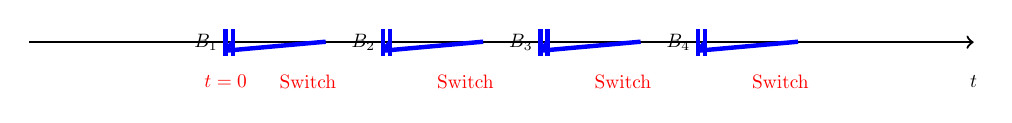
\begin{tikzpicture}[scale = 1, every node/.style={scale=.7}]
    \draw[->,thick] (-0.5,0)--(11.5,0);
    \foreach \i/\j in {2/B_1,4/B_2,6/B_3,8/B_4}{
        \draw[blue,ultra thick, shorten >=-2pt, shorten <=-2pt] (\i,-0.1)--(\i,.1)node[pos=0,anchor=south,sloped]{};
        \draw[blue,ultra thick] (\i,-0.1)--(\i+.09,0);
        \draw[blue,ultra thick, shorten >=-2pt, shorten <=-2pt] (\i+.09,-0.1)--(\i+.09,.1)node[pos=0,anchor=south,sloped]{};
        \draw[blue,ultra thick, shorten >=-2pt, shorten <=-2pt] (\i+.09,-0.1)--(\i+1.2,0);
        \node[right] at (\i+.6,-0.5) {\textcolor{red}{Switch}};
        \node at (\i-.25,0) {$\j$};
    }
    \draw (2,-.5) node {\textcolor{red}{$t=0$}};
    \node at (11.5,-0.5) {$t$};
    \end{tikzpicture}